\documentclass[a4paper, 11pt]{book}
\usepackage{/home/nicolas/Documents/Enseignement/Prepa/bpep/fichiers_utiles/preambule}
\newcommand{\qed}{\tag*{$\blacksquare$}}

\newcommand{\dsNB}{19}
\makeatletter
\renewcommand{\@chapapp}{Kh\^olles MPSI3 -- semaine \dsNB}
\makeatother

\toggletrue{corrige}  % décommenter pour passer en mode corrigé

% IMPORTS automatiques
\newcommand{\f}[2]{{
		\mathchoice
		{\dfrac{#1}{#2}}
		{\dfrac{#1}{#2}}
		{\frac{#1}{#2}}
		{\frac{#1}{#2}}
}}

\newcommand{\e}[1]{{}_{\text{#1}}}
\renewcommand{\a}[0]{\alpha}
\newcommand{\w}[0]{\omega}

\usepackage{physics}

 % fin des IMPORTS automatiques

\begin{document}

\chapter{Sujet 1\siCorrige{\!\!-- corrig\'e}}
\section{Question de cours}

Définir l'électronégativité d'un élément et donner (en le justifiant) son
évolution par colonne, par famille et globalement dans le tableau. Définir le
moment dipolaire d'une liaison, d'une molécule et la polarisabilité, et
déterminer le moment dipolaire de \ce{H2O} connaissant $p_{\ce{HO}} =
\SI{1.51}{D}$ et $\widehat{({\rm HOH})} = \ang{104.45}$.

\resetQ
\subimport{/home/nicolas/Documents/Enseignement/Prepa/bpep/exercices/TD/oscilloscope_analogique/}{sujet.tex}

\chapter{Sujet 2\siCorrige{\!\!-- corrig\'e}}
\section{Question de cours}

Définir ce que sont les interactions de \textsc{Van der Waals} et en donner
l'énergie potentielle générale. Présenter les 3 interactions que ce terme
regroupe~: nature, énergie potentielle, énergie de liaison. Donner la forme de
l'énergie potentielle des interactions répulsives, la forme de l'énergie
potentielle totale et indiquer sur le schéma comment se trouve la distance de
liaison et l'énergie de liaison. On donnera un ordre de grandeur des distances
d'interaction de \textsc{VdW}.

\resetQ
\section{Chute sur corde en escalade}
On étudie une grimpeuse qui chute. Une corde d'escalade de longueur $L_0$ peut,
en première approximation, être modélisée par un ressort de longueur à vide
$L_0$ et de raideur $k = \a/L_0$, avec $\a$ une caractéristique de la corde.

\begin{center}
    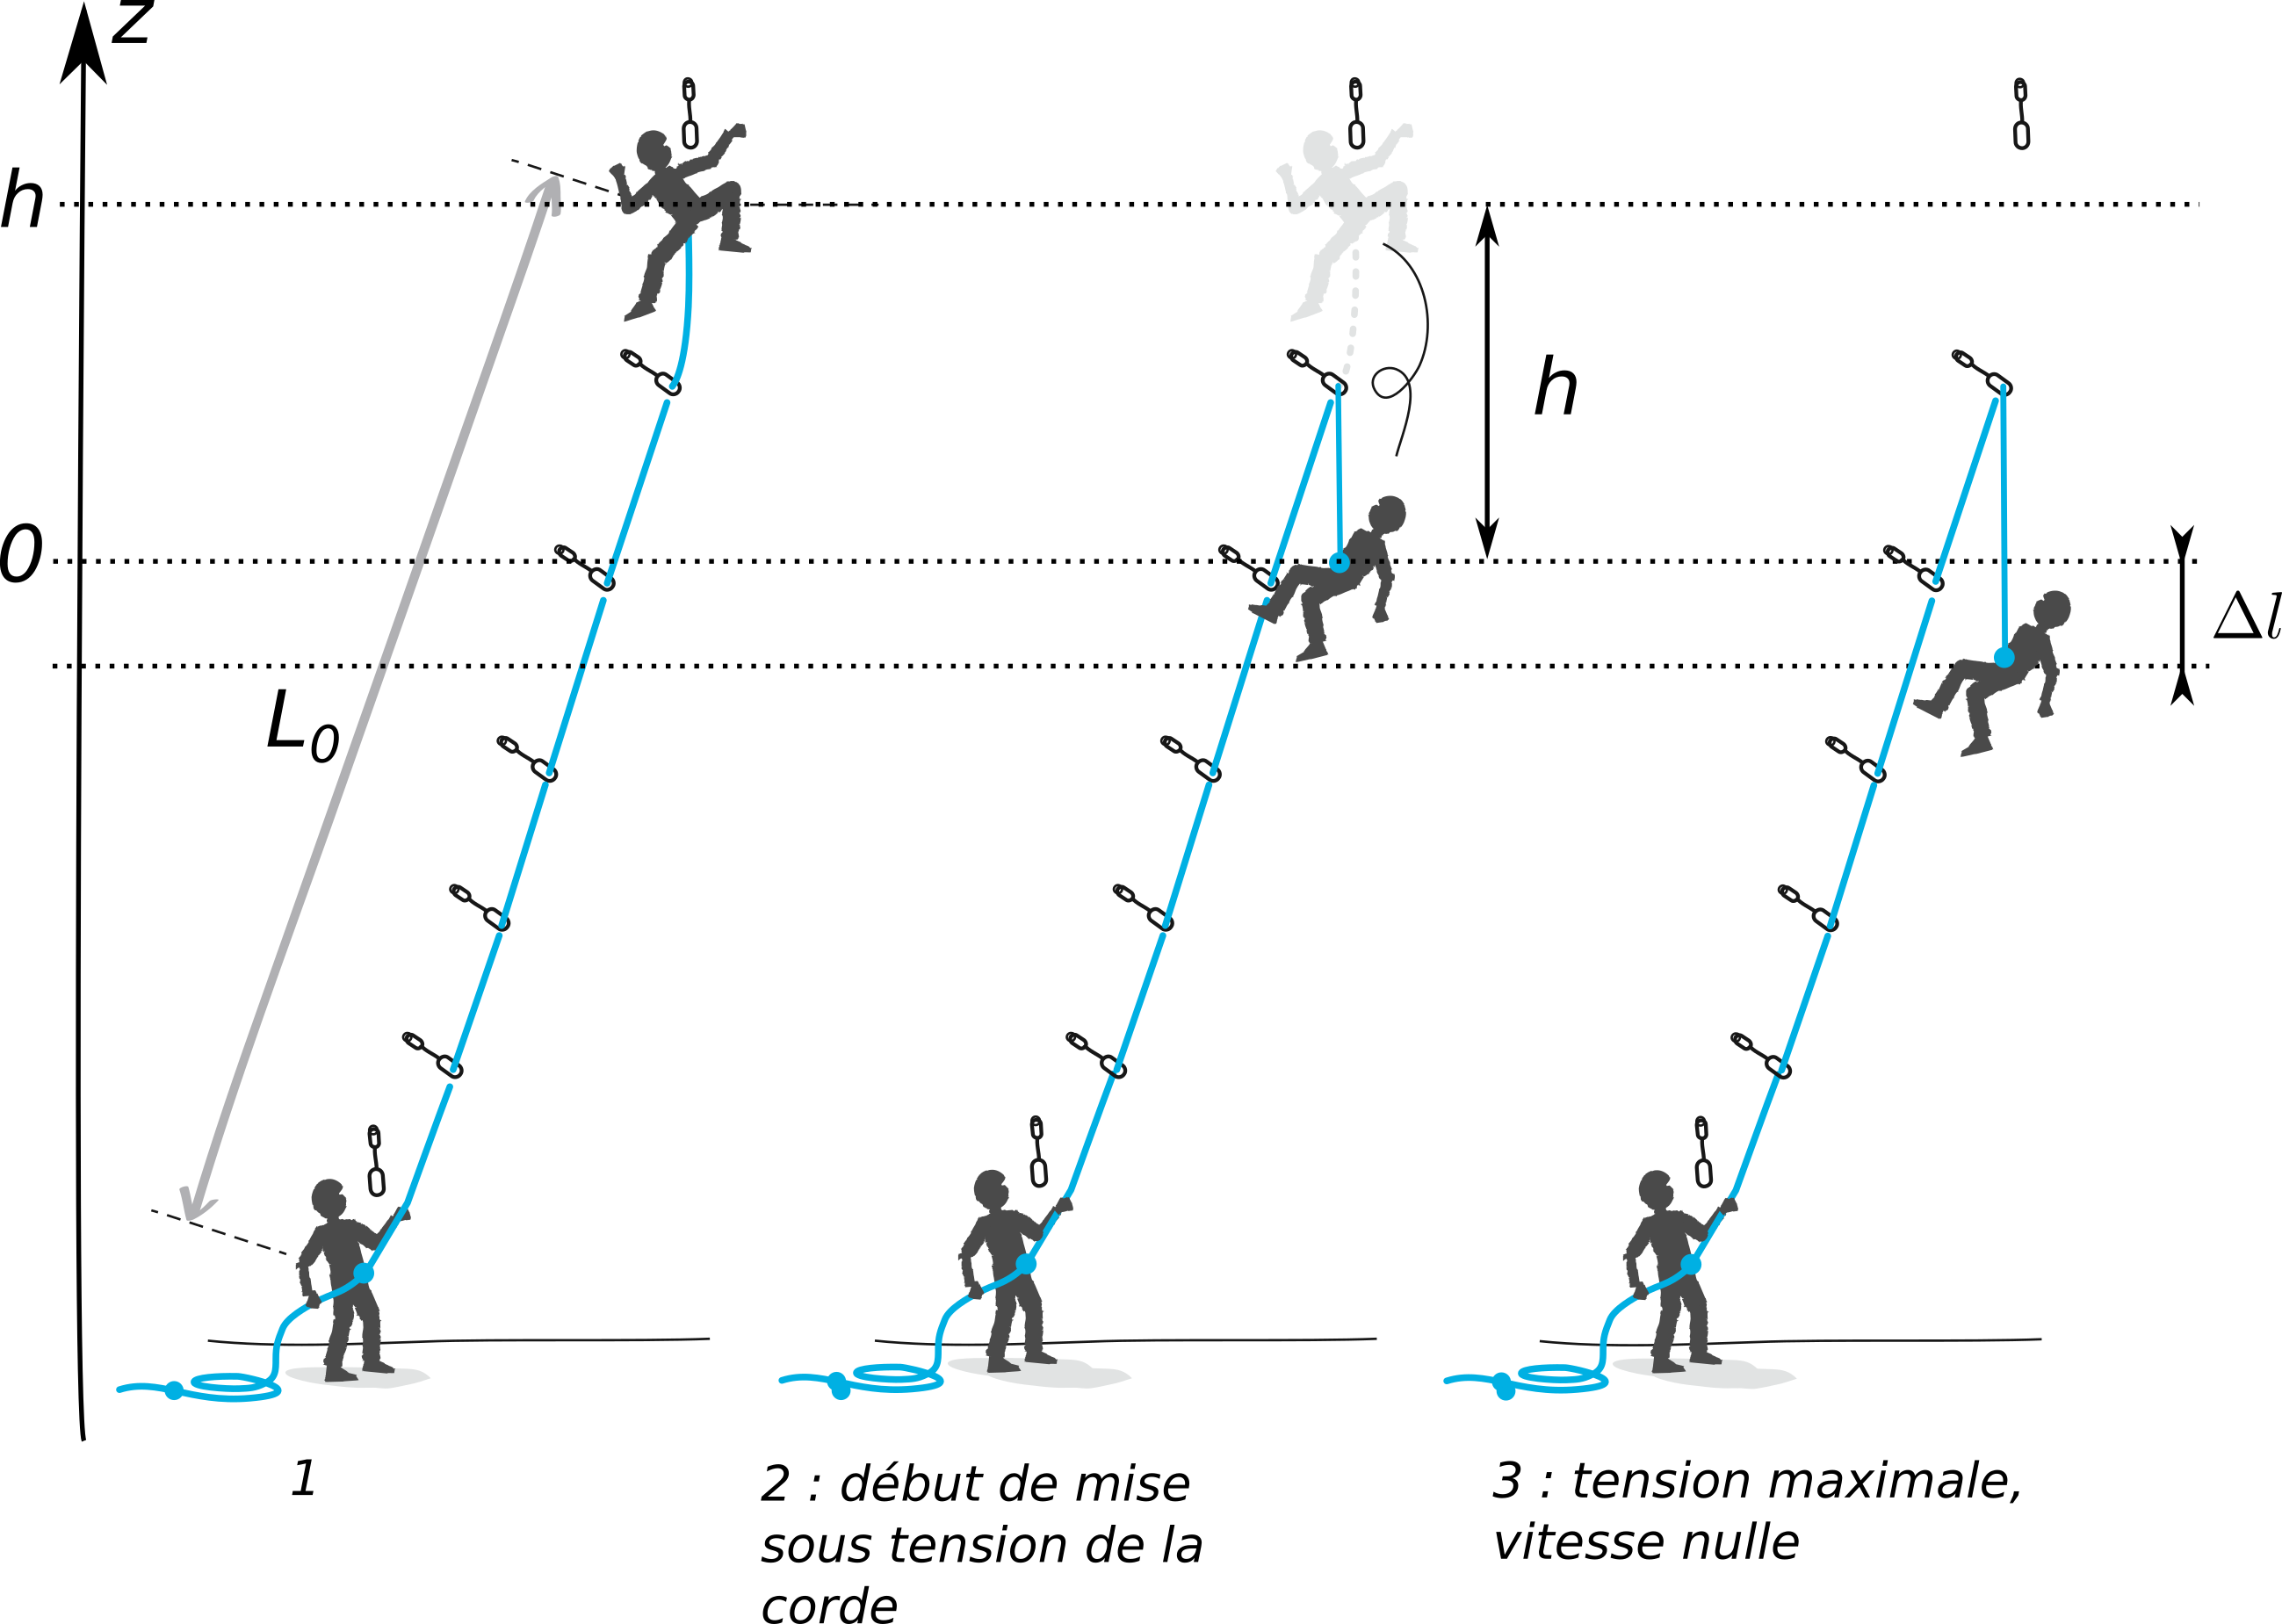
\includegraphics[width=.7\linewidth]{../../figures/ch18/chute_escalade-plain}
\end{center}

La grimpeuse est en chute libre sur une hauteur $h$ pendant laquelle la corde
n'est pas sous tension. La corde passe ensuite sous tension, et la chute se
poursuit sur une hauteur $\D l$. La vitesse de la grimpeuse devient ainsi nulle
au bout d'une hauteur totale de chute $h+\D l$.

On prendra $g = \SI{10}{m.s^{-2}}$, $\a = \SI{5.0e4}{N}$ et une grimpeuse de
masse $m = \SI{50}{kg}$. \bigbreak

\QR{À l'aide d'un bilan énergétique, donner l'expression de la vitesse
    maximale atteinte par la grimpeuse. Faire l'application numérique pour
une hauteur de chute $h = \SI{5}{m}$.}
{Pendant la chute libre, la grimpeuse ne subit que l'action du poids,
    qui est conservatif. On peut donc utiliser le TEM, avec~:
    \begin{itemize}[label=$\diamond$]
        \litem{Au début de la chute libre~:} $z = h$, $v=0 \Ra \Ec_{p,p} = mgh$ et
            $\Ec_c = 0$
        \litem{À la fin de la chute libre~:} $z = 0$, $v=v \Ra \Ec_{p,p} = 0$ et
            $\Ec_c = mv^2/2$.
    \end{itemize}
    D'où
    \begin{gather*}
        \frac{1}{2}mv^2 = mgh
        \Lra
        \boxed{v = \sqrt{2gh}}
        \qavec
        \left\{
            \begin{array}{rcl}
                g & = & \SI{10}{m.s^{-2}}\\
                h & = & \SI{5}{m}
            \end{array}
        \right.\\
        \AN
        \boxed{v = \SI{10}{m.s^{-1}}}
    \end{gather*}
}
\QR{Toujours à l'aide d'une méthode énergétique, donner l'expression de
    l'allongement maximal $\D l$ de la corde. On supposera $\D l \ll h$ afin
de simplifier le calcul.}
{On peut utiliser le TEM entre le point tout en haut et le point le
    plus bas, ou entre le point O et le point le plus bas. Faisons le
    premier cas~:
    \begin{itemize}[label=$\diamond$]
        \litem{Au début de la chute libre~:} $z = h$, $v=0 \Ra \Ec_{p,p} = mgh$ et
            $\Ec_c = 0$
        \litem{À la fin de la chute amortie~:} $z = -\D l$, $v=0 \Ra \Ec_{p,p}
            = -mg\D l$, \fbox{$\Ec_{p,el} = k\D l^2/2$} et $\Ec_c = 0$.
    \end{itemize}
    Ainsi,
    \begin{gather*}
        mgh = \frac{1}{2}k\D l^2 + mg(-\D l)
        \Lra
        mg(h+\underbracket[1pt]{\cancel{\D l}}_{\ll h}) = \frac{1}{2}k\D l^2
        \Lra
        \boxed{\D l = \sqrt{\frac{2mgh}{k}}}
        \qed
    \end{gather*}
    La solution trouvée est plausible~: homogène, augmente avec $m$, $h$ et
    $g$ mais diminue avec $k$.
}
\QR{Donner enfin l'expression de la norme de la force maximal $F_{\max}$
    qu'exerce la corde sur la grimpeuse. On introduira le facteur de chute
$f = h/L_0$.}
{En norme, une force de rappel s'exprime $F = k(\ell -\ell_0)$, soit
    ici
    \begin{gather*}
        F_{\max} = k\D l = \sqrt{2mgh\,k} = \sqrt{2mgh\frac{\a}{L_0}}
        \\\Lra
        \boxed{F_{\max} = \sqrt{2mg\a f}}
        \qed
    \end{gather*}
}
\QR{Au-delà d'une force de \SI{12}{kN}, les dommages sur le corps humain
    deviennent importants. Que vaut $F_{\max}$ pour une chute de $h =
\SI{4}{m}$ sur une corde de longueur $L_0 = \SI{4}{m}$~? Conclure.}
{On fait l'application numérique~:
    \begin{gather*}
        \qavec
        \left\{
            \begin{array}{rcl}
                m & = & \SI{50}{kg}\\
                g & = & \SI{10}{m.s^{-2}}\\
                \a & = & \SI{5.0e4}{N}\\
                f & = & \num{1}
            \end{array}
        \right.\\
        \AN
        \boxed{F_{\max} = \SI{10}{kN}}
    \end{gather*}
    Il n'y a donc pas de risque aggravé pour la grimpeuse avec cette chute.
}
\QR{Une chute d'un mètre arrêtée par une corde de \SI{50}{cm} est-elle
    plus ou moins dangereuse qu'une chute de \SI{4}{m} arrêtée par une corde
de \SI{8}{m}~?}
{Dans le premier cas, $f_1 = 2$~; dans le second, $f_2 = \num{0.5}$. Or,
$F_{\max}$ évolue en $\sqrt{f}$, donc plus $f$ augmente plus la force
subie augmente~: le premier cas est donc 2 fois plus dangereux que le
premier~!
}

\chapter{Sujet 3\siCorrige{\!\!-- corrig\'e}}
\section{Question de cours}

Savoir comment construire (pas connaître par cœur) les 4 premières
lignes du tableau périodique. Définir et placer les blocs $s$, $p$ et
$d$. Préciser les colonnes des familles des gaz rares, des halogènes et
des métaux alcalins. Placer le chlore \ce{Cl} ($Z = 17$) sur le tableau. Donner
le numéro atomique du magnésium \ce{Mg}, colonne 3 ligne 2. Établir leurs
configurations de valence et leur schéma de \textsc{Lewis}.

\resetQ
\subimport{/home/nicolas/Documents/Enseignement/Prepa/bpep/exercices/Colle/spectrometre_de_Dempster/}{sujet.tex}

\label{LastPage}
\end{document}
